Repeat-Copy is a task formulated in DeepMind's original DNC paper
\cite{graves2016hybrid} in order to test whether the architecture could
learn how to manage the external memory. The task itself isn't a difficult or
market demanding problem needing to be solved. The task simply has features in
which it can test the architecture of the DNC.

The Repeat-Copy task is described as follows. An agent receives as input
$n_{\textrm{min}}$ to $n_{\textrm{max}}$ many sequences of $m$ binary digits.
The agent is tasked to repeat the sequences of binary digits a given
$r_{\textrm{min}}$ to $r_{\textrm{max}}$ many times. Consider an example when
$n_{\textrm{min}} = 1$, $n_{\textrm{max}} = 10$, $m = 4$,
$r_{\textrm{min}} = 1$, and $r_{\textrm{max}} = 5$.
Then the agent receives between 1 to 10 sequences of 4 binary digits with
the task of repeatedly outputing those sequences of 4 binary digits between 1
to 5 times. A problem instance for this example would be to ask the agent to
output the following matrix 5 times:
$$
\begin{bmatrix}
    0 & 1 & 0 \\
    1 & 1 & 1 \\
    0 & 0 & 1 \\
    0 & 1 & 1
\end{bmatrix}
$$
where each of the $n$ many columns represent a sequence of $m$ binary digits.

The free gate in the DNC is active when the most recently read locations in
external memory can be freed. The allocation gate governs the strength to which
locations in external memory can be reused for new data. Training the DNC on
the Repeat-Copy task is forcing the model to learn when to free limited
external memory and reuse that freed memory to best take advantage of it.
Consider a task where the DNC receives a sequence of 10 random binary digits as
input and must repeat those 10 random binary digits as output. If the DNC uses
a feed-forward network with only an external memory of 10 locations, it must
learn to use the memory to only store data for each sequence at a time. The
DNC in this case doesn't have enough memory space to store all input it
receives to repeat. The results reported by DeepMind's DNC paper
\cite{graves2016hybrid} are such that the DNC learned how to manage external
memory as we would expect it must in order to succeed at the task. The free
gate becomes active while reading from external memory to immediately make that
space available for writing in later timesteps. The allocation gate becomes
active while receiving input to write the input into the freed locations.

The purpose of repeating DeepMind's Repeat-Copy results \cite{graves2016hybrid}
in our implementation has two primary reasons. Firstly, to reconfirm the DNC
model's ability to learn how to manage memory efficiently. Secondly, to ensure
our implementation of the DNC behaves similar to that of DeepMind's
before attempting further research. Our results on this task are shown in
Figure ~\ref{fig:repeatCopyResults} along with the comparable results provided
by DeepMind on the same task \cite{graves2016hybrid}.

\begin{figure}[!htb]
\begin{subfigure}{.9\textwidth}
    \centering
    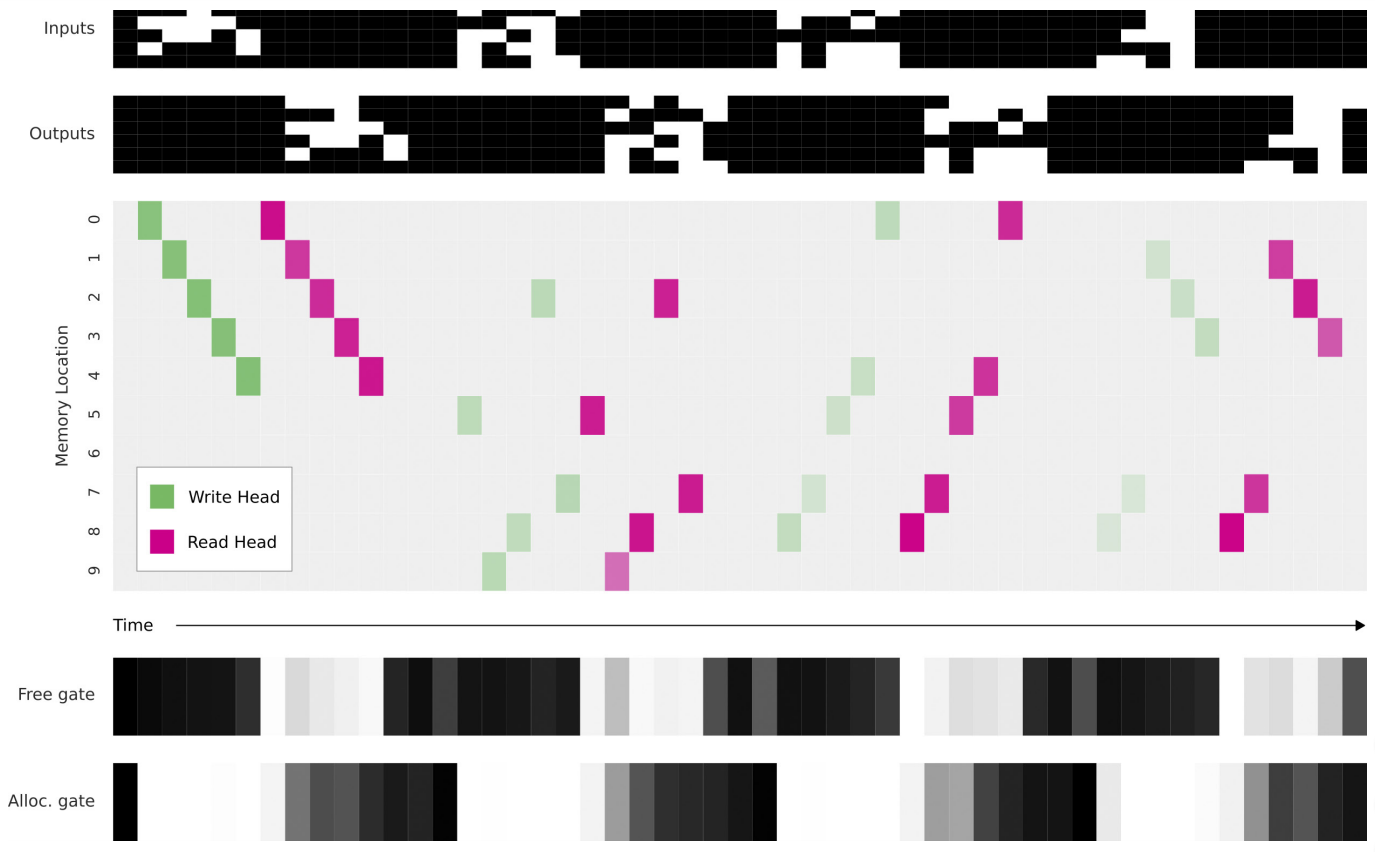
\includegraphics[width=1.0\linewidth]{../resources/DeepMind-RC-results.png}
    \caption{
        DeepMind's results on the Repeat-Copy task \cite{graves2016hybrid}.
    }
    \label{fig:repeatCopyResults_a}
\end{subfigure}
\begin{subfigure}{.9\textwidth}
    \centering
    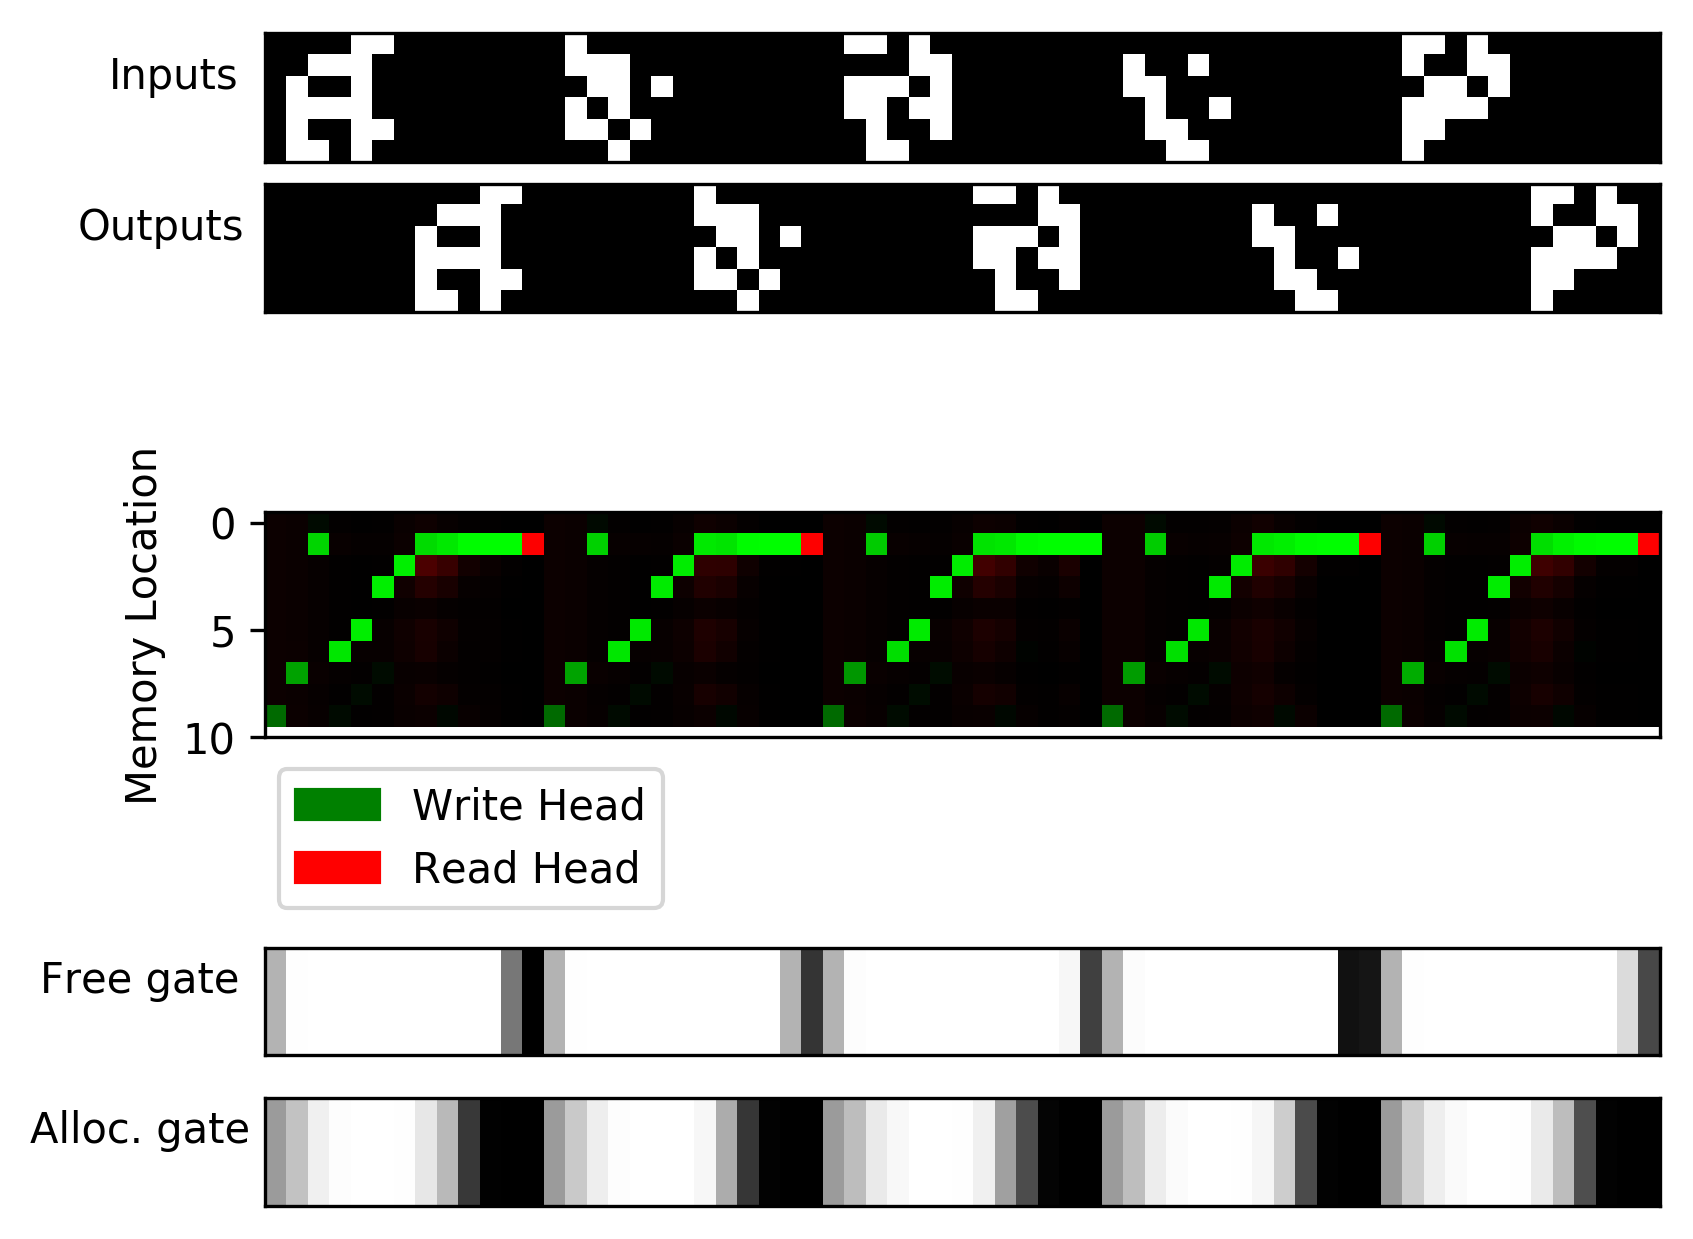
\includegraphics[width=1.0\linewidth]{../resources/RC-results.png}
    \caption{My results on the Repeat-Copy task.}
    \label{fig:repeatCopyResults_b}
\end{subfigure}
\caption{
    Both figures show the example input and the given outputs for a series of
    instance Repeat-Copy problems. The graphs are organized in increasing
    timesteps from the left column to the right column. The "Memory Locations"
    graph shows how active the corresponding read and write heads were during
    each timestep and at what memory locations. The "Free gate" and
    "Alloc. gate" graphs show how active the gate values were at each timestep
    where white means active and black means inactive.
}
\label{fig:repeatCopyResults}
\end{figure}

A DNC model instance was trained until almost complete accuracy in the
Repeat-Copy task. The task parameters are the same as that of DeepMind's for
their reported results ($n_{\textrm{min}} = n_{\textrm{max}} = 5$, $m = 6$, and
$r_{\textrm{min}} = r_{\textrm{max}} = 1$). In the case of our results shown in
Figure ~\ref{fig:repeatCopyResults_b}, all problems were solved correctly. The
model learned the task in a way where the write head was much more active than
the read head in most locations across all timesteps. Although small, the read
head is active during the output stage in the locations written to during the
input stage. You can see this by observing the faded red squares in the output
stage of each problem instance. This indicates the model is certainly writing
useful information to external memory as it receives input and also
reading/utilizing that useful information when it attempts to produce correct
output. This outcome is not as clear as it is within DeepMind's results
reported in Figure ~\ref{fig:repeatCopyResults_a}, but is still indicative that
the read and write heads are being properly utilized. DeepMind's graph of read
and write head activations are likely only showing the activation in select
locations to exaggerate this outcome. The results we report are the exact
read and right head activation values displayed as an rgb color. The write
head activation value controls the green channel of the color with the other
channels as zero. The read head activation value controls the red channel
of the color with the other channels as zero. This alone results in a graph
with greens, reds, and yellows because the read and write head is active at the
same locations for some of the timesteps. To make it more readable, we display
the color corresponding to the strongest activation while zeroing out the other
color channels.

Another important detail to point out about the memory locations graph shown
in Figure ~\ref{fig:repeatCopyResults_b} is that the same memory locations
are consistently used across problem instances. This strengthens the argument
that the DNC model can efficiently manage its external memory. Since the same
memory locations are being used, you would expect the results of a previous
problem instance to effect future outputs from the model. This however is not
the case since the model can solve the task with almost perfect accuracy on
random inputs. This enforces the idea that the DNC model learns to free up
unnecessary information stored in its external memory.

Recall that the free gate value's purpose is to control when memory locations
can be freed for future use. Our model reported in
Figure ~\ref{fig:repeatCopyResults_b} shows that the free gate is very active
for most of the timesteps with some inactivity occuring at the end of the
output stage. This pattern may mean that the model already freed up all the
memory locations at the end of the output stage and so no more locations need
to be freed. This pattern along with the reported read/write activity may also
mean that the model transfers information from one location to another as it
receives input. As it transfers information from one location to another, it
frees the first location since the information stored there is no longer
needed. The pattern may also indicate something else and provide no insight at
all. However, we can conclude that in same way the model learned to free up
memory locations that do not prevent the model from producing correct output.
This conclusion can be continued to say that the model most likely learned to
free locations it no longer needs so that those locations can be used again in
future problem instances. DeepMind reports
(Figure ~\ref{fig:repeatCopyResults_a}) that their model learned to primarily
free memory locations as the external memory is being read in the output stage.
This is because as the information is being read, it is no longer needed to
produce any future correct output.

Recall that the allocation gate becomes active on a timestep to assign a freed
memory location new information. Our model reported in
Figure ~\ref{fig:repeatCopyResults_b} shows that the allocation gate is most
active during timesteps the model receives input. When the model starts to
output information, the allocation gate's activation weakens. Without the
allocation gate being active during timesteps the model receives input, the
model would not be able to store new information about the input into the
external memory. The pattern of allocation gate activations reported for our
model is similar to that of DeepMind's reported in
Figure ~\ref{fig:repeatCopyResults_a}. Therefore we can conclude that our model
learned similar methods of storing information about the input to that
achieved by DeepMind's work.

The work we report reconfirms the DNC model's ability to learn how to manage
memory efficiently. It additionally provides support that our implementation
of the DNC behaves similar to that of DeepMind's. These two findings
successfully accomplishes the purpose of this repeated study and gives
motivation for further research.
